\chapter{Enol, Enolat, dan Reaksi Aldol}\label{ch:b2:enolates-aldol}

Setiap kali sebuah sel menguraikan glukosa, sebuah enzim memotong fosfat gula
berkarbon enam menjadi dua potongan berkarbon tiga: sebuah reaksi \omterm{def:b2:enolates-aldol:aldol}{aldol} yang
dijalankan mundur. Jika dijalankan maju, reaksi yang sama menyambungkan dua
senyawa karbonil menjadi satu, dan reaksi ini adalah cara yang paling banyak
dipakai kimiawan untuk membentuk ikatan karbon--karbon. Reaksi ini bertumpu
pada sebuah sifat yang baru disinggung oleh bab-bab sebelumnya: atom-atom
hidrogen di sebelah gugus karbonil bersifat asam, dan melepaskan salah
satunya mengubah karbon di samping karbonil menjadi nukleofil.

\begin{recall}
Jilid Tahun 1: $\mathrm pK_a$ dan reaksi predominan, karbanion, kendali
kinetik dan termodinamik, \omterm{def:b2:amines:nucleophilic-addition}{adisi nukleofilik} pada karbonil, eliminasi E1 dan
E2, hidrasi alkuna (sebuah \omterm{def:b2:enolates-aldol:tautomerism}{enol} yang mengalami penataan ulang).
\Cref{ch:b2:frontier-orbitals}: \omterm{def:b2:frontier-orbitals:ambident}{nukleofil ambiden}.
\Cref{ch:b2:acyl-substitution}: ester dan substitusi asil.
\end{recall}

\section{Tautomeri keto--enol}

\begin{definition}[Tautomeri]\label{def:b2:enolates-aldol:tautomerism}
Yang disebut \emph{tautomer}\index{tautomer} adalah isomer-isomer yang saling
berubah dengan berpindahnya sebuah hidrogen dan sebuah ikatan rangkap. Dalam
\emph{tautomeri keto--enol}\index{tautomeri keto--enol}, senyawa karbonil
yang mempunyai hidrogen pada karbon di sebelah karbonil (bentuk keto) berada
dalam kesetimbangan dengan \emph{enol}\index{enol}-nya, yaitu alkohol yang
dibawa oleh ikatan rangkap \ce{C=C}.
\end{definition}

\begin{omfigure}
\setchemfig{atom sep=2em}
\schemestart
\chemfig{H_3C-C(=[2]O)-CH_3}
\arrow{<=>[\ce{H+} atau \ce{HO-}][katalisis]}[,2.2]
\chemfig{H_3C-C(-[2]OH)=CH_2}
\schemestop
\par\vspace{6pt}

{\small Propanon dan \omterm{def:b2:enolates-aldol:tautomerism}{enolnya}, prop-1-en-2-ol. Asam (protonasi oksigen
karbonil, lalu lepasnya sebuah hidrogen $\alpha$) atau basa (pelepasan sebuah
hidrogen $\alpha$, lalu protonasi oksigen) mengatalisis perubahan timbal
balik itu; kesetimbangannya terletak jauh di sisi bentuk keto.}
\end{omfigure}

\begin{proposition}[Kandungan enol]\label{prop:b2:enolates-aldol:enol-content}
Aldehida dan keton sederhana hanya mengandung sekelumit \omterm{def:b2:enolates-aldol:tautomerism}{enol}; senyawa
1,3-dikarbonil seperti pentana-2,4-dion mengandung \omterm{def:b2:enolates-aldol:tautomerism}{enol} dalam proporsi yang
besar.
\end{proposition}

\begin{proof}[Argumen]
Ikatan \ce{C=O} lebih kuat daripada ikatan \ce{C=C} dengan selisih yang
lebih besar daripada selisih lemahnya ikatan \ce{O-H} dibandingkan dengan
ikatan \ce{C-H}: bentuk keto lebih disukai. Dalam senyawa 1,3-dikarbonil,
ikatan rangkap \omterm{def:b2:enolates-aldol:tautomerism}{enol} terkonjugasi dengan gugus karbonil kedua, dan \ce{OH}
\omterm{def:b2:enolates-aldol:tautomerism}{enol} membentuk ikatan hidrogen internal dengan oksigennya dalam cincin
beranggota enam: keduanya cukup menstabilkan \omterm{def:b2:enolates-aldol:tautomerism}{enol} sehingga \omterm{def:b2:enolates-aldol:tautomerism}{enol} menjadi
bentuk utama.
\end{proof}

Karena \omterm{def:b2:enolates-aldol:tautomerism}{enol} planar pada \ce{C=C}-nya, pusat stereogenik pada karbon $\alpha$
hilang setiap kali \omterm{def:b2:enolates-aldol:tautomerism}{enol} terbentuk: keton yang aktif secara optik dengan
pusat stereogenik di sebelah karbonilnya mengalami rasemisasi dalam asam
atau basa.

\section{Enolat}

\begin{definition}[Enolat]\label{def:b2:enolates-aldol:enolate}
Yang disebut \emph{karbon $\alpha$}\index{karbon alfa@karbon $\alpha$} sebuah
senyawa karbonil adalah karbon yang terikat pada karbon karbonil;
hidrogen-hidrogennya adalah \emph{hidrogen $\alpha$}\index{hidrogen alfa@hidrogen $\alpha$}.
Melepaskan salah satunya menghasilkan \emph{ion enolat}\index{ion enolat},
yang muatan negatifnya terbagi antara karbon $\alpha$ dan oksigen.
\end{definition}

\begin{proposition}[Keasaman hidrogen $\alpha$]\label{prop:b2:enolates-aldol:alpha-acidity}
Hidrogen $\alpha$ jauh lebih asam daripada ikatan \ce{C-H} biasa karena
\omterm{def:b2:enolates-aldol:enolate}{enolatnya} distabilkan oleh resonansi; hidrogen di antara dua gugus karbonil
cukup asam untuk dilepaskan oleh alkoksida atau bahkan hidroksida.
\end{proposition}

\begin{proof}[Argumen]
Dalam \omterm{def:b2:enolates-aldol:enolate}{enolat}, muatan negatif sebagian berada pada oksigen yang
elektronegatif; karbonil kedua di sisi lain mendelokalisasikannya pada dua
oksigen. Diukur dalam air, pentana-2,4-dion mempunyai $\mathrm pK_a =
9.0$ dan etil 3-oksobutanoat 10.7, sebanding dengan nitrometana (10.2), yang
anionnya distabilkan oleh gugus nitro dengan cara yang sama; keton
sederhana, dengan hanya satu karbonil, jauh lebih lemah --- terlalu lemah
untuk diukur keasamannya secara langsung dalam air.
% ledger: pka:acac, pka:acetoacetate, pka:nitromethane
\end{proof}

\begin{omfigure}
\setchemfig{atom sep=2em}
\schemestart
\chemfig{H_3C-C(=[2]O)-\chemabove{C}{\scriptstyle -}H_2}
\arrow{<->}
\chemfig{H_3C-C(-[2]\chemabove{O}{\scriptstyle -})=CH_2}
\schemestop
\par\vspace{6pt}

{\small Kedua struktur resonansi \omterm{def:b2:enolates-aldol:enolate}{enolat} propanon. Muatan negatifnya terbagi
antara karbon $\alpha$ dan oksigen: \omterm{def:b2:enolates-aldol:enolate}{enolat} adalah \omterm{def:b2:frontier-orbitals:ambident}{nukleofil ambiden}, yang
bereaksi pada karbon dengan sebagian besar elektrofil karbon.}
\end{omfigure}

\begin{definition}[Enolat kinetik dan termodinamik]\label{def:b2:enolates-aldol:kinetic-enolate}
Untuk keton dengan dua karbon $\alpha$ yang berbeda, \emph{enolat
kinetik}\index{enolat kinetik} adalah \omterm{def:b2:enolates-aldol:enolate}{enolat} yang terbentuk lebih cepat,
melalui pelepasan hidrogen dari sisi yang kurang terhalang dan kurang
tersubstitusi; \emph{enolat termodinamik}\index{enolat termodinamik} adalah
\omterm{def:b2:enolates-aldol:enolate}{enolat} yang lebih stabil, dengan ikatan rangkap yang lebih tersubstitusi.
\end{definition}

\begin{proposition}[Memilih enolat]\label{prop:b2:enolates-aldol:enolate-control}
Basa kuat dan meruah yang dipakai penuh pada suhu rendah (litium
diisopropilamida, LDA, pada \qty{-78}{\degreeCelsius}) membentuk \omterm{def:b2:enolates-aldol:kinetic-enolate}{enolat
kinetik} secara lengkap dan ireversibel; basa yang lebih lemah pada suhu
kamar (alkoksida dalam alkoholnya) membiarkan \omterm{def:b2:enolates-aldol:enolate}{enolat-enolat} saling berubah
dan terutama menghasilkan \omterm{def:b2:enolates-aldol:kinetic-enolate}{enolat termodinamik}.
\end{proposition}

\begin{proof}[Argumen]
LDA ($\mathrm pK_a$ diisopropilamina sekitar 36, jauh di atas nilai untuk keton)
mendeprotonasi secara lengkap dan cepat; pada suhu rendah, \omterm{def:b2:enolates-aldol:enolate}{enolatnya} tidak
terprotonasi kembali, dan deprotonasi yang lebih cepat, pada \ce{CH2} atau
\ce{CH3} yang mudah dijangkau, yang menentukan: kendali kinetik. Alkoksida
hanya melepaskan proton secara sebagian, \omterm{def:b2:enolates-aldol:enolate}{enolat-enolat} dan keton terus
bertukar proton, dan campuran kesetimbangannya lebih menyukai \omterm{def:b2:enolates-aldol:enolate}{enolat} yang
lebih tersubstitusi dan lebih stabil: kendali termodinamik (seperti dalam
jilid Tahun 1).
% ledger: ghs:LDA
\end{proof}

\section{Alkilasi enolat}

\omterm{def:b2:enolates-aldol:enolate}{Enolat} menyerang haloalkana primer melalui substitusi bimolekular, dan
membentuk ikatan \ce{C-C} baru pada karbon $\alpha$. Dengan hidrogen $\alpha$
senyawa 1,3-dikarbonil yang sangat asam, alkoksida sudah cukup, dan karbonil
tambahan itu dapat disingkirkan sesudahnya.

\begin{definition}[Dekarboksilasi]\label{def:b2:enolates-aldol:decarboxylation}
Yang disebut \emph{dekarboksilasi}\index{dekarboksilasi} melepaskan gugus
karboksil sebagai \ce{CO2}. Dalam \emph{sintesis ester
malonat}\index{sintesis ester malonat}, dietil propanadioat dideprotonasi,
dialkilasi, dihidrolisis menjadi asam propanadioat tersubstitusi, dan
didekarboksilasi dengan pemanasan, sehingga menghasilkan asam karboksilat
\ce{RCH2COOH}.
\end{definition}

\begin{proposition}[Dekarboksilasi yang mudah]\label{prop:b2:enolates-aldol:decarboxylation}
Asam $\beta$-keto dan asam propanadioat melepaskan \ce{CO2} pada pemanasan
lunak; asam karboksilat biasa tidak.
\end{proposition}

\begin{proof}[Argumen]
Karbonil yang berjarak dua ikatan dari gugus karboksil menerima hidrogen
\ce{COOH} dalam keadaan transisi siklik beranggota enam sementara \ce{CO2}
pergi: sebuah \omterm{def:b2:enolates-aldol:tautomerism}{enol} langsung terbentuk, lalu mengalami tautomerisasi. Tanpa
karbonil itu, karbanion yang akan ditinggalkan oleh lepasnya \ce{CO2} tidak
mendapat stabilisasi.
\end{proof}

\begin{definition}[Reaksi haloform]\label{def:b2:enolates-aldol:haloform}
Yang disebut \emph{reaksi haloform}\index{reaksi haloform} mengubah metil
keton \ce{RCOCH3}, dengan halogen dan hidroksida berlebih, menjadi
karboksilat \ce{RCOO-} dan haloform \ce{CHX3}.
\end{definition}

Setiap halogen yang dimasukkan membuat hidrogen-hidrogen $\alpha$ yang
tersisa lebih asam, sehingga gugus metil mengalami trihalogenasi; gugus
\ce{CX3-} lalu menjadi gugus pergi yang cukup baik untuk diusir oleh
hidroksida dalam substitusi asil. Dengan iodium, endapan kuning iodoform
merupakan uji untuk metil keton.

\section{Reaksi aldol}

\begin{definition}[Reaksi aldol]\label{def:b2:enolates-aldol:aldol}
Dalam \emph{adisi aldol}\index{adisi aldol}, \omterm{def:b2:enolates-aldol:enolate}{enolat} (atau \omterm{def:b2:enolates-aldol:tautomerism}{enol}) sebuah
senyawa karbonil beradisi pada gugus karbonil senyawa lain, sehingga
menghasilkan senyawa $\beta$-hidroksi karbonil, yaitu sebuah
\emph{aldol}\index{aldol}. Dalam \emph{kondensasi aldol}\index{kondensasi aldol},
aldol itu melepaskan air dan menghasilkan senyawa karbonil
$\alpha,\beta$-tak jenuh (enon atau enal).
\end{definition}

\begin{omfigure}
\setchemfig{atom sep=1.9em}
\schemestart
\chemfig{H_3C-CH=O} \+ \chemfig{^{-}CH_2-CH=O}
\arrow{->[adisi]}
\chemfig{H_3C-CH(-[2]O^{-})-CH_2-CH=O}
\schemestop

\medskip
\schemestart
\arrow{->[\ce{H2O}][$-$ \ce{HO-}]}
\chemfig{H_3C-CH(-[2]OH)-CH_2-CH=O}
\arrow{->[panas, basa][$-$ \ce{H2O}]}
\chemfig{H_3C-CH=CH-CH=O}
\schemestop
\par\vspace{6pt}

{\small Reaksi \omterm{def:b2:enolates-aldol:aldol}{aldol} etanal. \omterm{def:b2:enolates-aldol:enolate}{Enolat} beradisi pada molekul etanal kedua;
protonasi menghasilkan \omterm{def:b2:enolates-aldol:aldol}{aldol}, 3-hidroksibutanal. Pada pemanasan dengan basa,
sebuah hidrogen $\alpha$ dilepaskan dan hidroksida pergi dari karbon
$\beta$: but-2-enal, yang terkonjugasi.}
\end{omfigure}

\begin{proposition}[Mendorong reaksi aldol]\label{prop:b2:enolates-aldol:aldol-equilibrium}
\omterm{def:b2:enolates-aldol:aldol}{Adisi aldol} bersifat reversibel; dehidrasi, yang membentuk sistem
terkonjugasi, menarik reaksi ke arah produk kondensasi.
\end{proposition}

\begin{proof}[Argumen]
Dua molekul menghasilkan satu, sehingga \omterm{def:b2:reaction-free-energy:reaction-entropy}{entropi reaksinya} negatif, dan
ikatan \ce{C-C} yang baru hampir tidak melebihi ikatan $\pi$ \ce{C=O} yang
hilang: bagi banyak keton, $K$ kecil. Mengeluarkan \omterm{def:b2:enolates-aldol:aldol}{aldol} melalui dehidrasi
mempertahankan $Q < K$ untuk adisi; enon terkonjugasi yang terbentuk
terstabilkan dan, pada suhu tinggi, kenaikan entropi karena pelepasan air
makin mendukungnya. Reaksi kebalikannya, \omterm{def:b2:enolates-aldol:aldol}{retro-aldol}, adalah tahap yang
dipakai sel untuk memecah gula berkarbon enam.
\end{proof}

\begin{method}[Mengendalikan aldol silang]\label{met:b2:enolates-aldol:crossed-aldol}
\begin{enumerate}
  \item Pakailah satu pasangan tanpa hidrogen $\alpha$ (benzaldehida,
        metanal): pasangan itu hanya dapat menjadi elektrofil.
  \item Atau bentuklah \omterm{def:b2:enolates-aldol:enolate}{enolat} salah satu pasangan secara lengkap lebih
        dahulu (LDA, \qty{-78}{\degreeCelsius}), lalu tambahkan pasangan
        yang lain.
  \item Atau pakailah pasangan 1,3-dikarbonil, yang jauh lebih asam daripada
        pasangan yang lain.
  \item Utamakan aldehida sebagai elektrofil: aldehida lebih reaktif daripada keton.
\end{enumerate}
\end{method}

\begin{method}[Mengenali produk aldol]\label{met:b2:enolates-aldol:aldol-recognition}
\begin{enumerate}
  \item Carilah \ce{C=O} dengan \ce{OH} pada karbon yang berjarak dua atom ($\beta$), atau \ce{C=C}
        yang terkonjugasi dengan \ce{C=O}.
  \item Potonglah ikatan antara karbon $\alpha$ dan $\beta$: karbon $\beta$
        dulunya karbon karbonil (elektrofil), karbon $\alpha$ adalah karbon
        \omterm{def:b2:enolates-aldol:enolate}{enolat}.
  \item Periksalah bahwa kedua pasangan itu ada dan bahwa \omterm{def:b2:enolates-aldol:enolate}{enolatnya} dapat
        dibentuk secara selektif.
\end{enumerate}
\end{method}

\section{Kondensasi Claisen}

\begin{definition}[Kondensasi Claisen]\label{def:b2:enolates-aldol:claisen}
Dalam \emph{kondensasi Claisen}\index{kondensasi Claisen}, \omterm{def:b2:enolates-aldol:enolate}{enolat} sebuah
ester menyerang karbonil molekul ester lain dalam substitusi asil, sehingga
menghasilkan \emph{ester $\beta$-keto}\index{ester beta-keto@ester $\beta$-keto}
dan melepaskan alkoksida. Versi intramolekularnya, siklisasi Dieckmann,
menghasilkan ester $\beta$-keto siklik.
\end{definition}

\begin{proposition}[Pendorong kondensasi Claisen]\label{prop:b2:enolates-aldol:claisen-drive}
\omterm{def:b2:enolates-aldol:claisen}{Kondensasi Claisen} etil etanoat memerlukan satu ekuivalen penuh natrium
etoksida: kesetimbangannya tidak menguntungkan, dan reaksi itu didorong oleh
deprotonasi ester $\beta$-keto yang terbentuk.
\end{proposition}

\begin{proof}
Kondensasi itu sendiri, \ce{2CH3COOEt <=> CH3COCH2COOEt + EtOH}, mempunyai
tetapan kesetimbangan $K_1$ yang kecil. Ester $\beta$-keto ($\mathrm pK_a = 10.7$)
lalu dideprotonasi oleh etoksida (etanol, 15.9):
$K_2 = 10^{15.9 - 10.7} = 10^{5.2}$. Reaksi keseluruhannya, kondensasi
ditambah deprotonasi, mempunyai
$K_1K_2$, yang cukup besar bahkan untuk $K_1$ yang kecil; basanya terpakai
dan pengolahan asam menghasilkan
ester $\beta$-keto yang netral. Ester dengan hanya satu hidrogen $\alpha$, yang
produknya tidak dapat dideprotonasi, menghasilkan sedikit produk.
% ledger: pka:acetoacetate, pka:ethanol
\end{proof}

\begin{history}[Reaksi aldol, 1872]
\begin{minipage}[t]{0.18\linewidth}
\vspace{0pt}
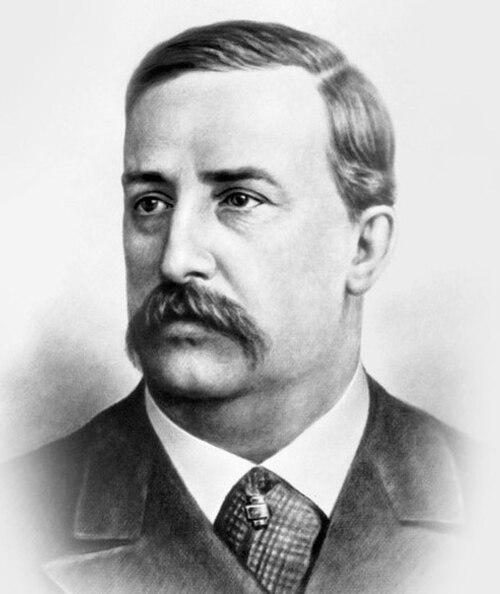
\includegraphics[width=\linewidth]{images/book3/borodin.jpg}
\end{minipage}\hspace{0.02\linewidth}%
\begin{minipage}[t]{0.18\linewidth}
\vspace{0pt}
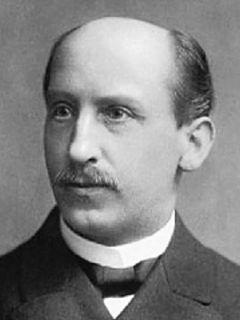
\includegraphics[width=\linewidth]{images/book3/claisen.jpg}
\end{minipage}\hfill
\begin{minipage}[t]{0.58\linewidth}
\vspace{0pt}
Reaksi \omterm{def:b2:enolates-aldol:aldol}{aldol} dideskripsikan pada tahun 1872 oleh Charles-Adolphe Wurtz dan,
secara terpisah, oleh Alexander Borodin, seorang kimiawan di Sankt-Peterburg
yang kini lebih dikenal sebagai penggubah \textit{Pangeran Igor}. Ludwig
Claisen memperluas kondensasi senyawa karbonil ke ester pada tahun 1887.
(Potret: Borodin, pembuat tidak diketahui, domain publik; Claisen, oleh
Veronica.villagrasa, CC BY-SA 4.0; Wikimedia Commons.)
\end{minipage}
\end{history}

\begin{safety}{\ghs[5mm]{GHS02}\,\ghs[5mm]{GHS05}\,\ghs[5mm]{GHS07}}
Natrium etoksida dan litium diisopropilamida bersifat korosif dan bereaksi
dengan air; larutan LDA mudah terbakar dan ditangani di bawah gas inert.
Benzaldehida dan propanon berbahaya dan mudah terbakar.
% ledger: ghs:NaOEt, ghs:LDA, ghs:benzaldehyde, ghs:acetone
\end{safety}

\section{Latihan}

\begin{exercise}[$\star$]\label{exo:b2:enolates-aldol:1}
Gambarlah \omterm{def:b2:enolates-aldol:tautomerism}{tautomer-tautomer} \omterm{def:b2:enolates-aldol:tautomerism}{enol} butanon dan sikloheksanon.
\end{exercise}

\begin{exercise}[$\star$]\label{exo:b2:enolates-aldol:2}
Urutkan menurut keasaman \ce{C-H} yang paling asam: propanon,
pentana-2,4-dion, etil 3-oksobutanoat, etana.
\end{exercise}

\begin{exercise}[$\star$]\label{exo:b2:enolates-aldol:3}
Tuliskan \omterm{def:b2:enolates-aldol:aldol}{aldol} dan produk kondensasi etanal dengan natrium hidroksida.
\end{exercise}

\begin{exercise}[$\star$]\label{exo:b2:enolates-aldol:4}
Tuliskan \omterm{def:b2:enolates-aldol:decarboxylation}{sintesis ester malonat} untuk asam heksanoat: haloalkana manakah yang diperlukan?
\end{exercise}

\begin{exercise}[$\star\star$]\label{exo:b2:enolates-aldol:5}
Gambarlah \omterm{def:b2:enolates-aldol:kinetic-enolate}{enolat kinetik} dan \omterm{def:b2:enolates-aldol:kinetic-enolate}{enolat termodinamik} 2-metilsikloheksanon serta
kondisi yang menghasilkan masing-masing.
\end{exercise}

\begin{exercise}[$\star\star$]\label{exo:b2:enolates-aldol:6}
Tuliskan produk \omterm{def:b2:enolates-aldol:aldol}{kondensasi aldol} silang benzaldehida dengan propanon (satu
ekuivalen masing-masing) dan jelaskan mengapa benzaldehida tidak
berkondensasi dengan dirinya sendiri.
\end{exercise}

\begin{exercise}[$\star\star$]\label{exo:b2:enolates-aldol:7}
Heksana-2,5-dion dalam basa mengalami \omterm{def:b2:enolates-aldol:aldol}{kondensasi aldol} intramolekular.
Cincin manakah yang terbentuk? Jelaskan pilihan di antara cincin-cincin yang
mungkin.
\end{exercise}

\begin{exercise}[$\star\star$]\label{exo:b2:enolates-aldol:8}
Tuliskan \omterm{def:b2:enolates-aldol:claisen}{kondensasi Claisen} etil etanoat dan produknya setelah pengolahan asam.
\end{exercise}

\begin{exercise}[$\star\star$]\label{exo:b2:enolates-aldol:9}
Manakah di antara senyawa berikut yang memberikan uji iodoform positif: propanon, pentan-3-on, etanal, asetofenon?
\end{exercise}

\begin{exercise}[$\star\star\star$]\label{exo:b2:enolates-aldol:10}
Tuliskan siklisasi Dieckmann dietil heksanadioat dan ukuran cincin produknya.
\end{exercise}

\begin{exercise}[$\star\star\star$]\label{exo:b2:enolates-aldol:11}
(\textit{R})-3-Metilpentan-2-on kehilangan aktivitas optiknya dalam natrium
hidroksida encer, tetapi (\textit{R})-4-metilheksan-2-on tidak. Jelaskan.
\end{exercise}

\begin{exercise}[$\star\star\star$]\label{exo:b2:enolates-aldol:12}
Usulkan jalur menuju 1,5-difenilpenta-1,4-dien-3-on, lalu menuju dienon
dengan dua gugus aril yang berbeda, dan jelaskan mengapa yang kedua lebih
sulit.
\end{exercise}

\section{Soal: Dibenzalaseton}

\begin{problem}[{Soal akhir pekan --- enolat propanon dan peran benzaldehida,
kedua kondensasi aldol, produk terkonjugasi, serta stoikiometri dan
rendemen sebuah preparasi}]
\label{pb:b2:enolates-aldol:1}
Preparasi (data latihan): \qty{2.1}{mL} benzaldehida dan \qty{0.75}{mL}
propanon diaduk dalam etanol dengan natrium hidroksida berair; kristal-kristal
kuning 1,5-difenilpenta-1,4-dien-3-on (dibenzalaseton) memisah; rendemen
75~\%. Massa jenis (\unit{g/cm^3}): benzaldehida 1.045, propanon 0.7845.
Massa molar (\unit{g/mol}): C 12.011, H 1.008, O 15.999.
% ledger: rho:benzaldehyde, rho:acetone, aw:C, aw:H, aw:O, ghs:dibenzalacetone

\medskip
\noindent\textbf{Bagian I --- Pasangan-pasangan.}
\begin{enumerate}
  \item Pasangan manakah yang mempunyai hidrogen $\alpha$? Berapa banyak?
  \item Gambarlah \omterm{def:b2:enolates-aldol:enolate}{enolat} propanon.
  \item Mengapa benzaldehida tidak dapat membentuk \omterm{def:b2:enolates-aldol:enolate}{enolat}?
  \item Mengapa propanon bereaksi dengan benzaldehida alih-alih dengan dirinya sendiri?
  \item Mengapa aldehida merupakan elektrofil yang lebih baik daripada keton?
  \item Mengapa hidroksida sudah cukup sebagai basa di sini?
\end{enumerate}

\medskip
\noindent\textbf{Bagian II --- Mekanisme.}
\begin{enumerate}[resume]
  \item Tuliskan adisi \omterm{def:b2:enolates-aldol:enolate}{enolat} pada benzaldehida.
  \item Tuliskan dehidrasi \omterm{def:b2:enolates-aldol:aldol}{aldol} yang terbentuk.
  \item Mengapa dehidrasi itu mudah di sini?
  \item Mengapa reaksi itu dapat terjadi untuk kedua kalinya?
  \item Tuliskan persamaan keseluruhannya.
  \item Apa yang mendorong reaksi itu sampai tuntas dalam preparasi ini?
\end{enumerate}

\medskip
\noindent\textbf{Bagian III --- Produk.}
\begin{enumerate}[resume]
  \item Berapa ikatan rangkap \ce{C=C} yang dimiliki dibenzalaseton, dan
        dengan konfigurasi apa (terutama)?
  \item Mengapa isomer (\textit{E},\textit{E}) lebih disukai?
  \item Hitunglah ikatan-ikatan $\pi$ yang terkonjugasi.
  \item Mengapa senyawa itu berwarna kuning sedangkan pasangan-pasangannya tidak berwarna?
  \item Apakah dibenzalaseton kiral?
\end{enumerate}

\medskip
\noindent\textbf{Bagian IV --- Stoikiometri dan rendemen.}
\begin{enumerate}[resume]
  \item Hitunglah massa molar benzaldehida, propanon, dan dibenzalaseton.
  \item Hitunglah jumlah kedua pereaksi.
  \item Pereaksi manakah yang menjadi pembatas?
  \item Hitunglah massa teoretis produk.
  \item Mengapa sedikit kelebihan benzaldehida lebih baik daripada kelebihan propanon?
  \item Apa yang akan dihasilkan oleh kelebihan propanon?
  \item Nyatakan massa dibenzalaseton yang diperoleh pada rendemen 75~\%.
\end{enumerate}
\end{problem}
